\documentclass[11pt]{llncs}
\usepackage{preamble}

\begin{document}
\import{./}{title.tex}
\thispagestyle{plain}
\import{./}{abstract.tex}


\section{Simplified mining model}

In order to be precise, while avoiding having to wave away network details and
message formats complicate our analysis, we describe in terms of interaction
with an oracle.

Instead of performing work (attempting to compute values with special images
under a hash function), simply interact with the oracle.

Intuitively, the oracle keeps track of the various puzzle graphs computed by
various parties, including the adversary.

\section{Puzzle Graph Oracle}

Puzzle graphs are directed graphs consisting of nodes, called puzzle solutions.

A puzzle solution is ``public'' or ``private''. Honest parties are able to see
the graph consisting of all the ``public'' puzzle solutions, and the (directed)
edges among them.

Puzzle solutions come with protocol-defined labels. The protocol may define
application semantics. For example, in our model the idea of ``included
transactions'' is a label. Our protocol will also include ``height'' as an
annotation. The protocol may define a ``validity'' condition.

The oracle interface is defined as follows:

    Graph is initially empty.

    on ReadPublicGraph():
        returns the graph consisting of all the public nodes and the (directed) edges between them

    on AddPuzzleSolution( label, edges ):
        Adds a new (public) node with the given label. Edges is a set of public nodes.
        A special label $\texttt{score}$ is chosen uniformly at random in the
        range $[0, 1]$.

    on AddPrivateSolution( label, edges ) from Adversary:
        same as AddPuzzleSolution, except the node is private. This may only be called by the adversary.


    on MakePublic( node ) from Adversary: change a node from private to public


    on PresentProof( recipient, nodes ):
        Presents a “pruned” graph, containing only nodes.
        Nodes is a subset of the nodes known to the oracle.
        The oracle sends to “recipient” the subgraph containing each node in $nodes$, all of the outgoing edge *labels* for each node.

Bounded rate oracle access:
    The number of oracle queries made by the adversary cannot exceed $f/N +
    O(1)$ of the number of oracle queries made by the honest parties.

\section{The Nakamoto protocol}

``Honest parties always work to extend the longest valid blockchain.''

Validity is defined inductively as follows:
- A puzzle solution with no outgoing edges is valid.
- A puzzle solution with a single outgoing edge to a valid puzzle solution is valid.

Properties (all of which hold when $f/N < 50\%$):
    Chain Quality:  the longest chain consists of puzzle solutions generated by honest nodes
    Prefix consensus: the longest valid chain includes a prefix that does not change.
        Since the adversary cannot add more puzzle solutions in a round than the honest chain, then the honest parties’ chain grows faster.

\section{Stateless Verification}

First, an arbitrary node from the graph (public or private) chain is chosen.
The verifier’s goal is to determine whether the node is ``stable,'' i.e. it is included in the longest chain.

Honest nodes and the adversary take turns presenting proofs to the verifier. The verifier does not use the Read() interface of the oracle, but simply accepts proofs sent to it by the oracle.

The verifier cannot tell which proofs are sent from honest parties or from the adversary!

Goals:
- (Common prefix) If the verifier accepts a transaction, then it will remain in the longest valid chain.
- (Liveness) If a node is included the chain, then after a short time GenerateProof() will produce a proof that the verifier accepts, regardless of proofs submitted by the adversary.

Bitcoin SPV Proofs:
	Simply pass the entire chain.
	In practice, the blockchain contains labels called “merkle roots”, and validity is based on whether merkle root corresponds to a set of valid transactions. Thus an SPV is substantially smaller than the entire blockchain including all the transactions. However, it grows linearly as the proof-of-work chain grows.

\section{Interactive Stateless Verification}

The Nakamoto protocol is modified as such:
- Every node still works to extend the longest valid chain.

A ``score'' is associated to, based on the number of leading 0-bits in the
``score'' label. Thus $X = score(n)$ is distributed according to a geometric distribution (with parameter 0.5).

Validity is modified as such:
- Each node contains several links. One is to the most recent puzzle solution, similar to the original protocol.
- Other links are to the most recent puzzle solution with $score(n) \geq
1$,  with $score(n) \geq 2$, and so on.

Present a proof-of-proof-of-work $(X, \pi)$. $\pi^{\rceil k}$

Disputing a false proof:
    If the transaction in question is *not* in the longest valid chain, but the adversary presents a proof.

Why is interaction needed?

Links along the layer.

\section{Compact SPV Proofs}

Similar to Kiayias, we utilize backlinks, in effectively the same structure.

Definitions:
$(\alpha, k)$ - Segment proof for $[start, end]$

Properties:
with high probability, at least puzzle solutions that contain ``start'' as a descendant

Efficiency:
	honest parties are able to produce a proof that contains fewer than $x$ blocks

Prefix proof.  for [end]
    The idea is to have successively larger proofs.

Let $A$ be a valid puzzle chain.

$A_{f}^{\mu}$, where $f \in A$, consists of the suffix of $A$ after
$f$, such that $n \in A$, $score(n) > \mu$, and $f \subset_A n$.

$\Pi_A[f]$  is defined by Alg 1.

$\Pi_{A}$ is a pruned version of A, defined by Alg 1.
$\Pi_{A}$ satisfies the following property:

\begin{equation*}
    \exists \mu \texttt{ such that } \Pi_{A}{f}^{\mu} = A_f^{\mu}
    \texttt{ and }
    |A_f^{\mu}| > k
    \texttt{ or } \mu
\end{equation*}

\section{Constructing non-interactive proofs}

\begin{figure}[h]
    \caption{The hierarchical blockchain. Existing blocks are shown in level 1.
    Higher levels have achieved a lower target (higher difficulty) during mining.}
    \centering
    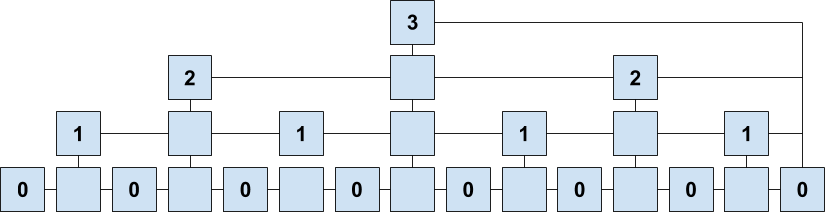
\includegraphics[width=\textwidth,keepaspectratio]{figures/hierarchical-ledger.png}
    \label{fig:hierarchy}
\end{figure}

\begin{figure}[h]
    \caption{The first of a series of interactive proofs-of-proofs-of-work.
    This proof is the only one that needs to be sent in case it goes
    unchallenged.}
    \centering
    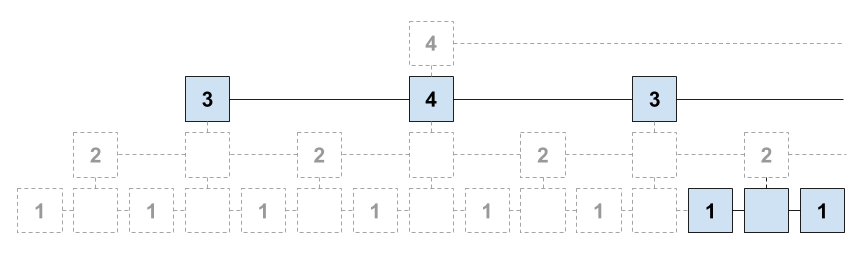
\includegraphics[width=\textwidth,keepaspectratio]{figures/interactive-popow.png}
\end{figure}

\begin{figure}[h]
    \caption{A non-interactive proof-of-work. Any challenges can be answered by
    the verifier directly by constructing a proof from the data in this proof,
    without interaction with the prover.}
    \centering
    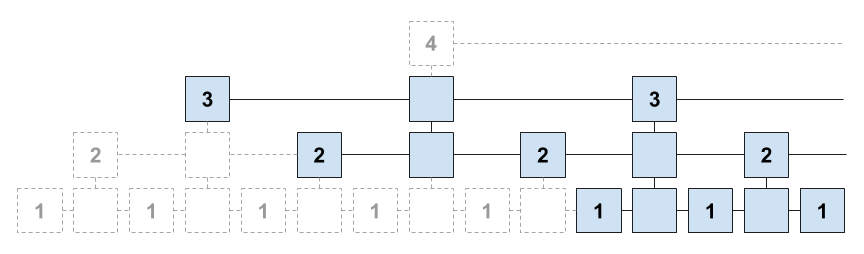
\includegraphics[width=\textwidth,keepaspectratio]{figures/non-interactive-popow.png}
\end{figure}

\import{./}{references.tex}
\end{document}
